\chapter{Theoretical Overview}
\label{chapter_theoretical_overview}
This chapter will explain terms and technologies associated with personalization and recommendation, mobile user interfaces and digital news applications, to form a basis of what is often used when creating a mobile news recommendation application.


\section{Mobile User Interface}
After the rise of the smart phone, mobile content consumption has seen an incredible growth and is still growing\cite{emarketer2012moretime}, making the mobile user interface more and more common to people everywhere. The focus here will be on the smart phone, and the iPhone in particular, but applies to a lot of other smart phones manufactured as well.

Mobile devices brings with it a lot of opportunities, but has its limitations as well, compared to a desktop computer, for instance. Mobile screens are smaller than PC screens and are often touch-based, making the design approach for a mobile user interface quite different.

A PC screen can normally hold more information in one view than a mobile device, so to display the same amount of information on a mobile screen, several views needs to be used and some form of navigation logic between them needs to be established.


\section{Personalization}

According to Cylogy, personalization is "the process of deciding - given a large set of possible choices - what has the highest value to an individual"\cite{personalization_overview}.

\cite{thurman2012future} defines it as "A form of user-to-system interactivity that uses a set of technological features to adapt the content, delivery, and arrangement of a communication to individual users’ explicitly registered and/or implicitly determined preferences."

So simple and a bit blunt stated: "give the users what they want, without them asking for it."

\section{Recommender System}
\label{theoretical_overview_recommender_system}
"The goal of a Recommender System is to generate meaningful recommendations
to a collection of users for items or products that might interest them."\cite{melville2010recommender}

Recommender systems are becoming widely used and is a necessary approach to deal with the ever growing information overload situation that are occurring nowadays. These systems can be found in many different domains, like online shopping, reading news, listening to music or streaming other types of visual media, like movies or series.

\subsection{Filtering}
When building a recommender system there are three main approaches to follow, namely content-based filtering, collaborative filtering or a hybrid of these two. 

\subsubsection{Content-based Filtering}
Content-based filtering is a filtering technique where the items proposed are chosen based on similar items to what the system thinks the user is interested in. The items have some sort of classifying meta data, that makes them comparable to other items, and the item with the best match to the user's profile will be the item proposed. The user profile can be built by extracting and classifying events from the user's click log, for instance, or by explicit data the user supplies in terms of categories of interest etc.

Content-based filtering is dependent on knowledge about the items to be able to classify and cluster them, and sophisticated methods based on machine learning and NLP are often used to fulfill this purpose. 


\subsubsection{Collaborative Filtering}
Collaborative filtering is a filtering technique that proposes items based on which items other similar users have been accessing. Often large amount of user data from other users' activities or preferences are gathered and analyzed and the users are put into segments based on their behavior. If a user from one segment accesses an item, this item can be proposed as a recommended item for another user within this segment.

An advantage of this approach as opposed to content-based filtering, is that collaborative filtering does not need to have an understanding of the item itself to be able to recommend it to a user. On the other hand, collaborative filtering often suffers from cold start\cite{lam2008addressing}, scalability and data sparsity\cite{huang2004applying} problems.

\subsubsection{Hybrid Filtering}
Hybrid filtering is an approach where content-based filtering and collaborative filtering are combined in some way, and it has shown that this approach is more effective in some cases, as presented in section \ref{related_work_personlized_news}.

One way of conducting the hybrid approach is to implement collaborative filtering and content-based filtering separately, and then combining them. Another way is to use some capabilities from one approach and add it to the other approach. One can also merge them together, and apply them as a single model.

\section{News Application}
A news application is an application where a user can access news digitally via the Internet from one or more news publishing sources. This application can be provided by the content publisher itself, or it can be provided by a third party redistributing the content.

News applications are becoming widely used, and the consumption of news are rapidly shifting towards accessing news online and via mobile devices (see figure \ref{pew_news_consumption_survey})\cite{pewresearch2012trends19912012}.

\begin{figure}[!htbp]
\centering
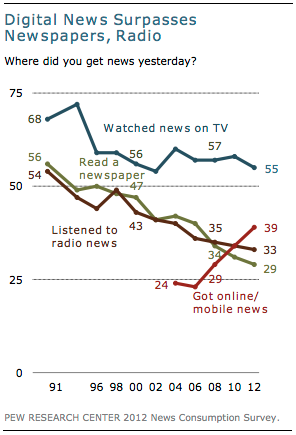
\includegraphics[width=70mm]{GFX/tech/pewNewsConsumptionSurvey.png}
\caption{The shifting of how people access news from 1991 to 2012 shown in percent of people asked.}
\label{pew_news_consumption_survey}
\end{figure}

\subsection{News Recommendation}
News recommendation is when a news application makes use of a recommender system to provide an online news reading user with a news service that are filtered or personalized to the user's preferences and likings.

A challenge with news recommendation, compared to for instance movie or music recommendation, is the freshness of the news. News have a short lifespan, and are best served fresh, making approaches like collaborative filtering a difficult task considering the cold start problem and data sparsity problem.



